\newpage
\chapter{ERM and PAC Learning}

In this chapter, we will introduce the concept of \textbf{Empirical Risk Minimization} (ERM) in which to frame learning problems, the notion of inductive bias, and the main results of algorithmic learnability, encapsulated in the definition of \textbf{Probably Approximately Correct} (PAC) Learning and of complexity of a set of hypothesis, namely
VC-dimension and Rademacher complexity.

\section{Empirical Risk Minimization}

We begin by considering a supervised learning setting in which the \textbf{input space} $X$ is a subset of $\mathbb{R}^n$, and the \textbf{output space} $Y$ can be real-valued (e.g., $Y = \mathbb{R}$), binary (e.g., $Y = \{0,1\}$), or a finite set of classes (e.g., $Y = \{0,1,\ldots,K\}$). In this probabilistic framework, each input-output pair $(x,y)$ is drawn from a joint probability distribution
$$
p(x,y) \;\in\; \mathrm{Dist}(X \times Y),
$$
often referred to as the \emph{\textbf{data generating distribution}}. 

By definition, this distribution factors into the marginal $p(x)$ and the conditional $p(y \mid x)$, so that
$$
p(x,y) \;=\; p(x)\,p(y \mid x).
$$

Because $p(x)$ and $p(y \mid x)$ describe how inputs and outputs are related, it is helpful to write them explicitly. The marginal distribution of $x$ is
$$
p(x) \;=\; \int p(x,y)\,dy,
$$
while the conditional distribution of $y$ given $x$ is
$$
p(y \mid x) \;=\; \frac{p(x,y)}{p(x)}.
$$

A typical dataset $D$ in supervised learning consists of $N$ input-output pairs drawn independently from $p(x,y)$. We denote this as
$$
D \sim p^N(x,y),
$$
which means
$$
D \;=\; \{(x_i, y_i) \,\mid\, i = 1, \dots, N\},
$$
where each $(x_i, y_i)$ is sampled according to the joint distribution $p(x,y)$. 

In many cases, we assume that $p(y \mid x)$ depends on some unknown function of $x$. Formally, one might write
$$
p(y \mid x) \;=\; p\bigl(y \mid f(x)\bigr),
$$
where $f$ is the function we aim to learn. The central objective in supervised learning—through methods such as empirical risk minimization—is to find or approximate this function $f$ by using the observed data $D$.

\section{Risk and Empirical Risk}

$h \in \mathcal{H} \quad x,y \sim p(x,y)$

\textbf{\textit{loss function}} $l(x,y,h) \in \mathbb{R_{\ge 0}}$, 

\begin{itemize}
    \item 0-1 loss: $l(x,y,h) = \mathbb{I}(h(x) \neq y)$, eith $y \in \{0, 1\}$.
    \item squared loss: $l(x,y,h) = (h(x) - y)^2$, with $y \in \mathbb{R}$.
\end{itemize}

We have a probabilistic process, so we have some inputs that are more likely than others. If a model makes a mistake on a more likely input, it should be penalized more.

\begin{definitionblock}[Risk]
The \textbf{\textit{risk}} (or \textbf{\textit{generalization error}}) is defined as:
$$
R(h) = E_{x,y \sim p(x,y)}[l(x,y,h)]
$$ 
\end{definitionblock}

\textbf{Risk minimization principle:}

The goal is to find the hypothesis $h$ that minimizes the risk.
$$
\text{find } h^* \in \mathcal{H} \text{ such that } h^* = \mathrm{arg\,min}_{h \in \mathcal{H}} R(h)
$$

\begin{definitionblock}[Empirical Risk]
The \textbf{\textit{empirical risk}} (or \textbf{\textit{training error}}) is defined as:
$$
\hat R = \dfrac 1N \sum_{i=1}^N l(x_i, y_i, h)
$$
\end{definitionblock}


\textbf{Empirical risk minimization principle:}

The goal is to find the hypothesis $h$ that minimizes the empirical risk.
$$
\text{find } h^*_D = \mathrm{arg\,min}_{h \in \mathcal{H}} \hat R(h)
$$

\subsection{Bias Variance Trade-off}

In this section, we want to analyze the generalization error and decom-
pose it according to the sources of error that we are going to commit.

In what follows, we will use the squared loss (hence we will focus on
regression problems). Considering $h \in \mathcal H$, an explicit expression of the generalization error committed when choosing hypothesis $h$ is:
$$
R(h) = E_p[l(x,y,h)] = \int \int (h(x) - y)^2 p(x,y) dx dy
$$

\newtheorem{theorem}{Theorem}

\begin{theorem}
    The minimizer of the generalization error $R$ is:
    $$
    \boxed{ g(x) = E[y|x] = \int y p(y|x) dy }
    $$
    so that $g = \mathrm{arg\,min}_h R(h),\ if\ g \in \mathcal H$
\end{theorem}

We can rewrite the risk as:
$$
R(h) = \underbrace{\int (h(x) - g(x))^2 p(x) dx}_{=\ 0 \quad iff \quad h(x) = g(x)} + \overbrace{\iint (g(x) - y)^2 p(x,y) dx dy}^{\text{independent of }h \text{: intrinsic noise}}
$$



$$
\begin{array}{rl}
E_D[R(h^*_D)]
& = \underbrace{\int ( E_D[h^*_D(x) - g(x)])^2 p(x) dx}_{bias^2} \\
& + \underbrace{\int E_D[(h^*_D(x) - E_D[h^*_D(x)])^2 p(x) dx]}_{variance} \\
& + \underbrace{\iint (g(x) - y)^2 p(x,y) dx dy}_{noise}
\end{array}
$$

\section{ERM and Maximum Likelihood}

Given a dataset $D = \{(x_i, y_i)\}_{i=1, \dots, m}$ s.t. $D \sim p^m, p = p(x,y)$

We factorize the data generating distributions as: $p(x,y) = p(x) p(y|x)$ and we make an hypothesis on $p(y|x)$, trying to express this conditional probability in a parametric form:

$$p(y|x) = \underbrace{p(y|x, \theta)}_\text{\small parametric family of distributions}$$

where $\theta$ is the parameter of the model.

We consider the log Likelihood:
$$
L(\theta; D) = log \prod_{i = 1}^{m} p(y_i|x_i, \theta) = \sum_{i = 1}^m \log p(y_i | x_i, \theta)
$$

Then we apply the maximum likelihood principle, according to which:

$$
\Theta_{\text{ML}} = \argmax{\theta} L(\theta; D) = \argmin{\theta} - L(\theta; D)
$$

It holds that:

$$
\begin{array}{rcl}
    \argmin{\theta} - L(\theta; D) &
    = & \argmin{\theta} - \dfrac 1m \displaystyle\sum_{i=1}^m \log p(y_i | x_i, \theta) \\
    & \approx & \argmin{\theta}\ \mathbb{E}_{p(x,y)}[-\log p(y | x, \theta)]
\end{array}
$$

since the avarage is an empirical approximation of the expectation.

\begin{definitionblock}[Cross-Entropy]
    The \textbf{\textit{cross-entropy}} is defined as:
    $$
    - \dfrac 1m \sum_{i = 1}^m \log p(y_i | x_i, \theta)
    $$
\end{definitionblock}

\section{KL Divergence}

From a physical point of view, entropy is a measure of disorder of a system, while from a probabilistic point of view is a measure of "surprise".

A measure, called \textbf{self-information}, of a probability distribution {p(x)} is given by the negative of the logarithm of the probability of the event:

$$
I(x) = - \log p(x)
$$

Indeed, if $p(x) = 1$, then $I(x) = 0$, while if $p(x) = 0$, then $I(x) = \infty$. In general, the more rare the event is, i.e. the lower is $p(x)$ the higher is the self-information, i.e. the larger is $- \log p(x)$.

In an information-theoretic sense, the \textbf{entropy} is a measure of the information that is carried by a random phenomenon, expressed as the expected amount of self-information that is conveyed by a realization of the random phenomenon.

Entropy is formally defined as:

$$
\mathbb{H}[p] = \mathbb{E}_{p}[-\log p(x)] = \quad 
\begin{array}{ll}
- \int p(x) \log p(x) dx & \quad \text{(if } x \text{ is continuous)} \\[10pt]
- \sum_i p(x) \log p(x_i) & \quad \text{(if } x_i \text{ is discrete)}
\end{array}
$$

In the discrete case, the maximum entropy is achieved for the uniform distribution and it is equal to $\log K$, with $K$ number of events that can happen. In the continuous case, for a fixed variance, the distribution that maximizes entropy is the Gaussian. The entropy is always 0 if we have a deterministic distribution.

\begin{definitionblock}
The \textbf{Kullback-Leibler divergence} is a measure of how one probability distribution diverges from a second, expected probability distribution. It is defined as:
$$
\mathbb{KL}[p||q] = \int q(x) \log \dfrac{q(x)}{p(x)} dx
$$
\end{definitionblock}

Intuitively, we are taking a sort of expected difference between $p$ and $q$, expressed in terms of a log odds ratio. It tells us how different the two distributions are. The larger the KL divergence, the more different the two distributions are.

\subsubsection{Properties of KL divergence}
\begin{itemize}
    \item $\mathbb{KL}[p||q] = 0$ iff $p = q$.
    \item $\mathbb{KL}[p||q]$ is a convex function of $q$ and $p$ and $\mathbb{KL}[p||q] \ge 0$
    \item $\mathbb{KL}$ is non-symmetric: $\mathbb{KL}[p||q] \neq \mathbb{KL}[q||p]$
    \item $\mathbb{KL}[p||q] = -H[q] - \mathbb{E}_{p}[\log q(x)]$, where the first term is the entropy of $q$ and the second term is the cross-entropy.
\end{itemize}

\vspace{10em}
\dots
\vspace{10em}

\subsection{KL Divergence and Maximum Likelihood}

Consider a dataset: $\underline{x} : x_1, ..., x_N$:

\begin{definitionblock}
The \textbf{empirical distribution} is defined as:
$$
p_{emp}(x) = \dfrac 1N \sum_{i=1}^N \mathbb{I}(x - x_i)
$$
\end{definitionblock}

It is an approximation of the input data generating function $p(x)$. Practically, the more observations we have, the better the approximation.

Given a distribution $q$, we can compute:

$$
\mathbb{KL}[p_{emp}||q] = \mathbb{E}_{p_{emp}}[-\log q(x)] - \mathbb{H}[p_{emp}] = \underbrace{- \dfrac 1N \sum_{i=1}^N \log q(x_i)}_{- \frac 1N L(q, D)} - \mathbb{H}(p_{emp})
$$

if $q = q_0$, this is $- \frac 1N L(\theta)$ plus a constant. Hence, maximising $L(\theta)$ is equivalent to minimizing the KL divergence between the empirical distribution and the model distribution. This means that we can always rephrase maximum likelihood in terms of cross-entropy.

\section{PAC Learning}

Consider an hypothesis set $\mathcal{H}$ with the realizability property, i.e. $\exists \bar h \in H \text{ s.t. } p_{x,y}(\bar h(x) = y) = 1$, since $y \in \{0, 1\}$ then $\exists f : X \rightarrow Y \text{ s.t. } p_{x,y}(\bar h(x)) = f(x)$ (that is, our hypothesis set contains the true function).

\begin{definitionblock}
    A realizable hypothesis set $\mathcal{H}$ is \textbf{PAC-learnable} \textit{iff} $\forall \varepsilon, \delta \in (0,1), \forall p(x,y)$, $\exists m_{\varepsilon, \delta} \in \mathbb{N} \text{ s.t. } \forall m \ge m_{\varepsilon, \delta}, \forall D \sim p^m, |D| = m$, then:

    $$
    p_D(R(h_D^*) \le \varepsilon) \ge 1 - \delta
    $$
\end{definitionblock}

\vspace{10em}
\dots
\vspace{10em}

\begin{definitionblock}
    Given an hypothesis set $\mathcal{H}$ (not necessarily realizable) and an algorithm $A$, $\mathcal{H}$ is \textbf{agnostic PAC-learnable} iff $\forall \varepsilon, \delta \in (0,1), \forall p(x,y), \exists m_{\varepsilon, \delta} \in \mathbb{N} \text{ s.t. } \forall D \sim p^m, |D| = m \ge m_{\varepsilon, \delta}, \text{ then:}$

    $$
    p_D(R(h_D^A) \le \min_{h \in \mathcal{H}} R(h) + \varepsilon) \ge 1 - \delta 
    $$

    being $h_D^A$ the result of applying $A$ to $\mathcal{H}$ and $D$.
\end{definitionblock}

In other words, there exists a number of samples $m_{\varepsilon, \delta}$ such that the probability of the algorithm $A$ to find a hypothesis $h$ whose risk is close to the minimum risk ($\le \varepsilon$) is at least $1 - \delta$.

We have a bound of generalization error in terms of $\varepsilon$ and $\delta$ and, in order to achieve this bound, we need to have enaugh data points. Tipically:

\begin{itemize}
    \item $m_{\varepsilon, \delta}$ depends polinomially on $\dfrac 1\varepsilon$ and $\dfrac 1\delta$ (since we want the number of observations to increase moderately with the complexity of the problem)
    \item $A$ should run in polinomial time.
\end{itemize}

\vspace{10em}
\dots
\vspace{10em}

\section{VC Dimension}

Consider a class of hypothesis functions $\mathcal{H} = \{h : X \rightarrow \{0, 1\}\}$, and a set of points $C = \{c_1, ..., c_N\} \subseteq X$ of input points.

Define $\mathcal{H}_C = \{h(c_1), ..., h(c_N) \mid h \in \mathcal{H}\}$, the set of all tuples of Booleans obrained by applying all possible hypothesis functions $h \in \mathcal H$ to all points in $C$. We say that $\mathcal{H}$ \textbf{shatters} $C$ iff $|\mathcal{H}_C| = 2^m$.

Practically, this means that for any label assignment to points in $C$, we havce a function in our hypothesis set which is able to match such an assignment. Namely, we can exactly describe every possible dataset with inputs in $C$.

\begin{definitionblock}[VC Dimension]
    The \textbf{Vapnik-Chervonenkis (VC) dimension} of $\mathcal{H}$ is the size of the largest set $C$ that can be shattered by $\mathcal{H}$, i.e. the largest set $C$ such that $\forall \{0, 1\}^N$ can be realized by $\mathcal{H}$:

    $$
    VC dim(\mathcal{H}) = \max \{m | \exists C \subseteq X, |C| = m \text{ s.t. } \mathcal{H} \text{ shatters } C\}
    $$
\end{definitionblock}

\begin{tipsblock}[Just one point]
    In calculating the VC dimension, it is enaugh that \textit{we find one set of} $m$ points that can be shattered, it is not necessary to prove that all sets of $m$ points can be shattered.
\end{tipsblock}

\subsection{VC dimension and PAC learning}

In what follows, we will explore the reasons why VC dimension is crucial for PAC learnability.

\vspace{1em}

\newtheorem{proposition}{Proposition}
\begin{proposition}
    If $\mathcal{H} shatters C, |C| \ge 2m$, then we cannot learn $\mathcal{H}$ with $m$ samples.
\end{proposition}

Hence, there will be an assignment of $m$ samples to classes in which we are going to commit a large error.

\begin{figure}[H]
    \centering
    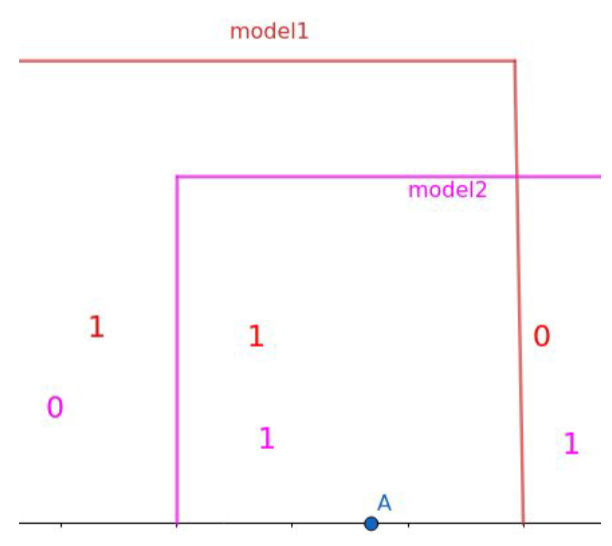
\includegraphics[width=0.5\textwidth]{assets/PAC_and_VC.png}
    \caption{Visual interpretation of the theorem: it is impossible to train a model of type $\mathcal{H_{a+}}$, with only a point $A$ with known classification (suppose 1) because the points differ from $A$ could have any classification.}
\end{figure}